\documentclass[fleqn,10pt]{wlscirep}
\usepackage[utf8]{inputenc}
\usepackage[T1]{fontenc}
\usepackage{graphicx}
\graphicspath{{../}}
\usepackage{url}
\usepackage{float}
\renewcommand{\JournalTitle}[1]{#1}

\title{Scaffolding Students-AI Dialogue: A Framework for Safe Educational Interactions}

\author[1,2,+,*]{Olga Muss}
\author[2,+,X]{Luca M. Leisten}
\author[3]{Charles Edouard Bardyn}
\affil[1]{Université de Neuchâtel, Switzerland}
\affil[2]{ETH Zurich, Switzerland}
\affil[3]{AI Swiss, Switzerland}

\affil[*]{olga.muss@unine.ch}
\affil[X]{lleisten@ethz.ch}

\affil[+]{these authors contributed equally to this work}

\keywords{AI safety, education technology, language models, reliability engineering, verification, quality education (SDG 4)}

\begin{abstract}
Adolescents are the fastest and largest age group adopting the use of Large Language Models (LLMs), models that were not specifically developed with their educational, emotional, and developmental needs in mind. Safe, adapted, and appropriate LLMs are essential for AI literacy, as well as for the safe and beneficial use in educational settings and beyond. In this paper, we present Steered Contextual AI Framework for Orchestrating Learning Dialogue (SCAFFOLD), a layered reliability framework that surrounds text/speech generation with external verification, targeted repair, and safe fallback that could work with any LLM while enabling data privacy. Grounded in pedagogical and developmental science of learning, in particular in the fact that learning requires effort, SCAFFOLD is designed to preserve productive effort, supporting active human-AI collaboration. SCAFFOLD starts by designing the interaction for a given context and goal, and then defines guidance and checks to be implemented. It distinguishes deterministic checks from probabilistic checks. We test SCAFFOLD in a classroom deployment with 12--16-year-old students using a LLM-powered social robot in a multi-user interaction of co-creation of a mnemonic on a topic covered previously. Students first interacted with a prompt-only LLM and then with SCAFFOLD during a learning intervention. Our results show more activity, engagement and on-topic talk with SCAFFOLD compared to the prompt-only LLM. Additionally, students' co-creation efforts with SCAFFOLD predicted their post-test knowledge scores, showing potential of the framework to support engagement, social interactions, and learning.
\end{abstract}

\begin{document}

\flushbottom
\maketitle
\thispagestyle{empty}

\section*{1 Introduction}

Generative Artificial Intelligence (AI) in the form of Large Language Models (LLMs) used in AI chatbots has been transformative in the last few years with a rapid adoption of AI chatbots by the general public and particularly young users \cite{InternetMatters2025, CommonSense2025, Hashem2025, Microsoft2024}. In Switzerland, 84\% of 14--19-year-olds report regular use of generative AI, the highest usage of any other age group, while only 60\% of 30--49-year-olds and less than 40\% of 50--69-year-olds report regular AI use \cite{WIP-CH2025}. Similar numbers come from the United Kingdom, in which 67\% of 15--17-year-olds and 53\% of 9--11-year-olds report regular use of AI chatbots \cite{InternetMatters2025}. This is no surprise, since AI chatbots are now embedded in apps that children and adolescents regularly use, such as Snapchat, WhatsApp, TikTok, or Instagram \cite{Ofcom2025, Vosloo2025}.

The risks of using LLMs are numerous, particularly for children and adolescents who are still developing, going from data privacy concerns and unsafe responses to attachment, cognitive atrophy and over-trust \cite{Neugnot2024, Kurian2025, UNESCO2021, VIOLA2017, Yu2025}. While society as a whole needs to address these issues, the educational sector faces specific challenges, as it simultaneously has to educate students about AI technologies and protect them from harm \cite{UNCRC1989} -- a duty even more critical when considering that children's knowledge is limited and their brains are still developing \cite{Gogtay2004}. In particular, in the age of generative AI, when the risks of cognitive atrophy, cognitive delegation, offloading or surrender are present \cite{Shaw2026}, the need to preserve effort necessary for learning would require supporting active human-AI collaboration, or ``human-AI co-thinking'' \cite{BardynForthcoming}. To fulfill the potential benefits of generative AI tools for education and young people's lives, we need to ensure that these tools are safe and developmentally adapted to their users \cite{UNESCO2021}.

Existing approaches to AI safety in education are insufficient: technical safeguards like content filters can block harmful outputs but don't ensure pedagogically sound interactions, while pedagogical frameworks cannot reliably steer unpredictable LLM behavior. Addressing this requires bridging conceptual and technical work: defining pedagogically appropriate students-AI interactions and developing methods to reliably implement them. Here we present a methodology that is both conceptual and technical - \textbf{Steered Contextual AI Framework for Orchestrating Learning Dialogue (SCAFFOLD)} - which goal is to enable alignment of pedagogical goals with technical feasibility in the educational context of students-AI interactions. We first present the general concept of SCAFFOLD, highlighting its potential, and then present the results of a pilot study with 12-16 year-old students. The contributions of this paper are:

\begin{itemize}
\item \textbf{A novel methodological framework}: \textbf{SCAFFOLD} consists of a modular system of frames that sits between students and the LLM, analyzing inputs, shaping prompts with safeguards, verifying outputs against pedagogical requirements, and triggering repairs or fallbacks when needed, thereby enabling reliable implementation of pre-designed educational interactions, independently of the LLM model and enabling data privacy and integration of the science of learning.
\item \textbf{Empirical validation in authentic educational settings}: We piloted the framework in classroom deployment with 12-15-year-old students using an LLM-powered social robot in a multi-user co-creation task. Results demonstrated that students were significantly more active, engaged, and on-topic with the framework compared to baseline LLM interaction.
\item \textbf{Evidence for learning potential}: Higher levels of student co-creation predicted post-test knowledge scores, suggesting the framework's potential to support both engagement and learning outcomes.
\item \textbf{Open-source implementation}: The complete modular system for co-creating a mnemonic in multi-user interactions with an AI, including balanced turns management, contribution tracking, phases and time management, is available open-source, enabling the community to build upon and extend this work for diverse educational contexts.
\end{itemize}

\section*{2 A framework for safe LLM interactions}

The need for external verification is grounded in a foundational principle from reliability engineering: reliability is not found, it is built, it requires error detection and correction at every stage. Generative AI inverts the traditional computing paradigm. Where classical software offered accuracy at the cost of rigid programming, generative AI offers effortless creation at the cost of reliability \cite{Xu2025, BardynWhitepaper2025}. Generating a plausible answer now costs fractions of a cent, while verifying whether that answer is safe, accurate, and pedagogically appropriate remains cognitively expensive \cite{BardynWhitepaper2025, Xu2025}.

LLMs are inherently probabilistic: they produce statistically likely continuations, not verified truths. A safety instruction that holds early in a dialogue may be overridden by later context, which is why prompting alone is insufficient as a reliability mechanism for educational settings. Given this fundamental unreliability, two verification paths exist: machine verification (algorithmic checks that provide strict guarantees in formal domains such as mathematics or code compliance) \cite{Gou2024, Madaan2023} and human verification (necessary for open-ended tasks involving judgment, context, and intention) \cite{Korthals2026}. Most educational tasks --- analysis, synthesis, creative expression, ethical reasoning --- fall outside the scope of purely algorithmic verification. They depend on the learner's specific situation, goals, and developmental stage.

SCAFFOLD addresses the space between these two poles: interactions that can be partially formalised through explicit pedagogical design. By translating educator-defined interaction parameters into a combination of deterministic checks (code-enforced, with guarantees) and probabilistic checks (AI-judged, with calibrated confidence), the framework surpasses reliability of pure prompting, while acknowledging that certain properties remain inherently probabilistic.

Several lines of research inform SCAFFOLD's design. We briefly review approaches to LLM output control, AI in education, and the regulatory context.

\subsection*{2.0.1 LLM guardrails and output control}

Recent work has proposed multiple strategies for steering LLM behaviour. Constitutional AI \cite{Bai2022} embeds behavioural principles directly into the training process, improving alignment but offering no per-turn enforcement once the model is deployed. NeMo Guardrails \cite{Rebedea2023} introduces programmable rails that intercept input and output at runtime, enabling control of topics and safety filtering. Self-refinement methods, such as Reflexion \cite{Shinn2023} and CRITIC \cite{Gou2024}, ask the model to critique and revise its own output. While each technique addresses a specific failure mode, these were not designed for educational settings where interactions must simultaneously satisfy pedagogical objectives, developmental constraints, and multi-user group dynamics. SCAFFOLD integrates these techniques (constitutional prompting in the prompt-shaping step, post-hoc validation akin to guardrails, and self-refinement through the correct--reverify loop) within a unified pipeline that is driven by an explicit pedagogical interaction design. The key differentiator is that SCAFFOLD begins from the learning activity, not from the model: educators specify what the interaction should achieve and what behaviour is acceptable, and the framework translates those specifications into enforceable checks.

\subsection*{2.0.2 AI in education}

Intelligent Tutoring Systems (ITS) have a long tradition of adaptive educational interaction, typically relying on domain models and student models to personalise instruction \cite{VanLehn2011}. More recently, commercial products such as Khanmigo (Khan Academy) and Duolingo Max have integrated LLMs into educational platforms. These systems generally rely on internal prompting strategies and proprietary safety layers whose implementation is not publicly documented, making independent verification difficult. SCAFFOLD differs in three respects: (i) it is model-agnostic and open-source, allowing external scrutiny; (ii) it distinguishes deterministic from probabilistic checks, making the reliability profile of each constraint explicit; and (ii) it places pedagogical interaction design --- not prompt engineering --- at the centre of the process, with the goal to enable educators to shape AI behaviour without coding expertise.

\subsection*{2.0.3 Regulatory context}

The EU AI Act classifies AI systems used in education as high-risk, requiring conformity assessments, human oversight, and transparency \cite{EUAIAct2024}. While the Act specifies what must be achieved, it offers limited guidance on how. SCAFFOLD provides a candidate implementation pathway: its layered verification architecture offers traceable, auditable decision-making at each turn, its deterministic checks provide documented guarantees, and its frame-based design supports the transparency and human oversight requirements that the regulation demands.

For these reasons, SCAFFOLD builds on a major preliminary step: first designing the desired interaction, and then uses several techniques to steer the LLMs' behavior. The overview of the flow of information and design is presented in \textbf{Figure 1}. We first outline the concept, explaining what we mean by designing an AI - student interaction, then describe the technical implementation of the interaction design into a modular and layered framework.

\begin{figure}[htbp]
\centering
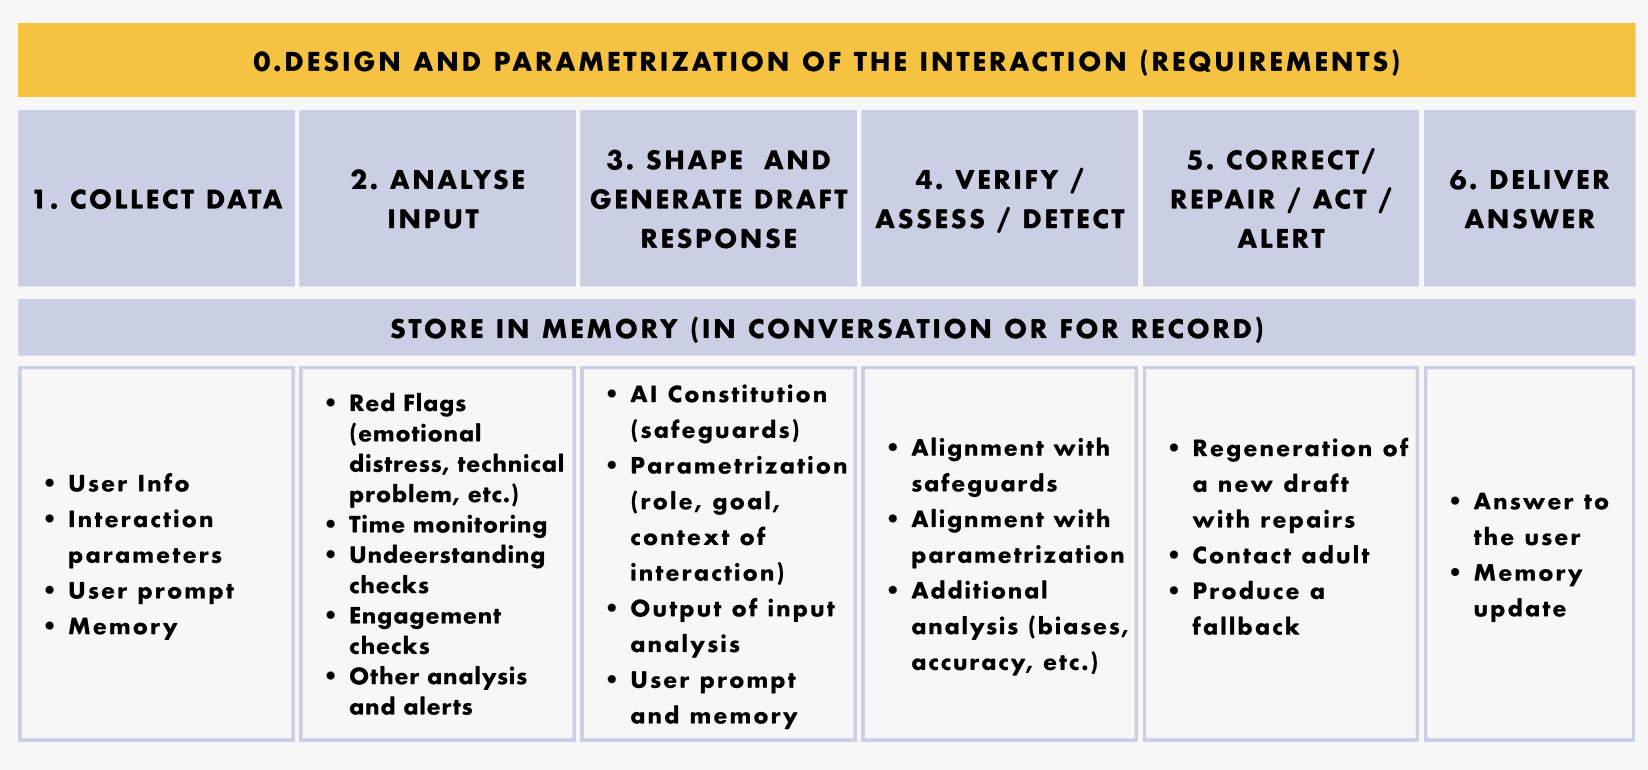
\includegraphics[width=\linewidth]{Images for manuscript/Figure 1}
\caption{Overview of the SCAFFOLD method for each turn in a multi-turn conversation}
\label{fig:overview}
\end{figure}

\subsection*{2.1  Designing a Students-AI interaction}

A human to human interaction is grounded in context, past experiences, time and location, guiding social norms and the behavior of the interlocutors \cite{Clark1996}. In interactions with AI the context is defined by the users' prompts which may or may not include additional information such as memory from past conversations or documents. In educational settings, the goal is learning and supporting development, often both in cognitive, sensory-motor and socio-emotional terms, and a successful integration of AI should at least support some of these learning goals \cite{ZawackiRichter2025}. The science of learning is a crucial guide for identifying effective pedagogical principles, considering individual differences and learning dynamics \cite{Bjork1994, Deci1985, Roediger2011, Dunlosky2013, Weinstein2018, Dukes2019}. Scaffolding, feedback timing, adaptive support, multisensory input, retrieval and spacing, metacognition and many other tools can inform technology-mediated learning environments for designing better learning interactions \cite{Macina2023, ZawackiRichter2025}.

Lesson planning and activity design requires educators to define the learning goals, the context, the pedagogical strategy, the activity and the content to cover, the flow, the structure, the rules, the assessment, all while considering students zone of proximal development and the needed scaffolding \cite{Wood1976, Vygotsky1978}. In a similar way, an AI-supported learning activity needs to be defined in terms of the above mentioned elements of a learning activity \cite{ZawackiRichter2025} and also in terms of the desired behavior of the LLM \cite{Neugnot2026}. For example, if a student asks for an answer to a question, should the LLM tell the answer, ask the student what he or she thinks the answer is, ask for the student's reasoning, provide a hint, or ask a metacognitive question? One can leave the decisions to the LLMs or define scaffolding, by designing the desired interaction. Likely only the latter solution could capture the benefits of the cognitive and social learning theories mentioned above.

A learning interaction, with or without AI, is a dynamic process involving feedback loops that reinforce or discourage certain behaviors in a multi-turn dialogue. It is therefore necessary, in the context of students-AI interactions to design these with the desired flow in mind, building on the science of learning and pedagogy. It is also necessary to steer LLM's behavior at each turn depending on what is happening in the interaction. Since it is impossible to define all possible behaviors in all situations, the goal could rather be to set key elements of an AI-interaction in a specific learning activity and improve these at each iteration.

\begin{figure}[htbp]
\centering
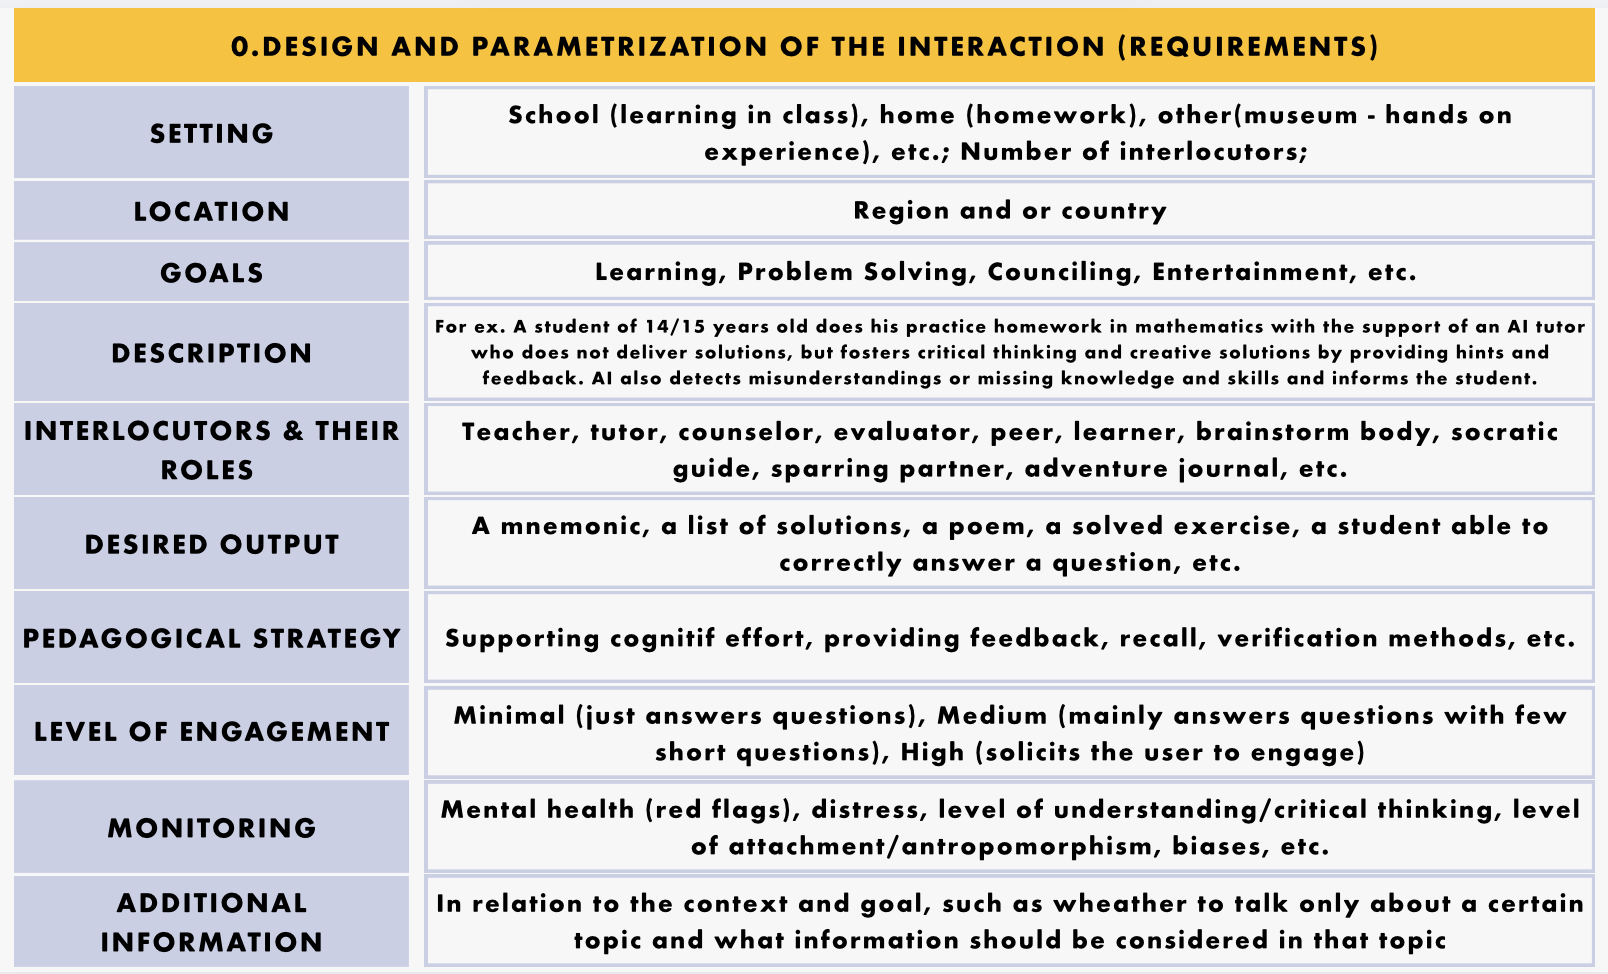
\includegraphics[width=\linewidth]{Images for manuscript/Figure 2}
\caption{Elements of a parametrization of an interaction}
\label{fig:parametrization}
\end{figure}

Drawing on established instructional design elements (learning goals, context, pedagogical strategy, assessment) and extending them to AI-mediated learning, Figure 2 illustrates categories of parameters that could be considered when designing students-AI interactions. These examples demonstrate the design space available to educators rather than constituting a validated taxonomy. The first type defines the context of the interaction, such as its setting, location, goals, interlocutors and description, allowing to integrate cultural and linguistic specificities. The second group of parameters defines the behavior of the LLM, such as desired output, pedagogical strategy, level of engagement, etc. A third group defines what happens in the background, such as what data is collected and how, what analysis needs to happen, etc. Finally, comes the learning material to consider and any other considerations not included previously.

A brainstorming activity of 15-year-olds in the context of creative writing could start with the LLM asking questions about students' ideas, instead of generating ideas for them. Or, an LLM may be used to monitor students' participation in a socratic seminar, where the LLM could invite less-active students to participate more. Homework support, work organization, language development, assessment support, and other possibilities all require a definition of specific elements of behavior. Students-AI interaction design can become an opportunity to critically reflect about the pedagogical practices and students' learning.

The interaction could be defined in a wide way and be suitable in many situations or it could be very specific to a certain use-case. Most of these parameters could be defined either as a freely formatted prompt or the users could be guided through a set of choices. The exception is the monitoring and assessment that requires more background definition and testing to be considered accurate, which, once developed, could be added to the toolbox in a modular way.

The interaction design described above produces a set of requirements: the learning goals, the desired LLM behaviour, the constraints that must be enforced, and the data to be collected. The next section describes how SCAFFOLD translates these requirements into a modular, enforceable technical architecture that operates at each conversational turn.

\subsection*{2.2 Steering LLM behavior at each turn}

The behavior of an LLM depends on its training data, size, structure of the model, its reinforcement learning from human feedback (RLHF), eventually some fine-tuning using labelled data, and the input to the model \cite{Ouyang2022, Bai2022, Zhao2023}. Here we are working with existing LLMs and therefore cannot modify the models themselves, only the inputs. Several strategies exist such as (i) prompt engineering and constitutional prompting \cite{Bai2022}, which consists in adding instructions to the user's prompt to introduce safeguards or steer reasoning as in chain-of-thought technique \cite{Wei2023}; (ii) post-hoc filters \cite{Rebedea2023}, which are answer validation checks; (iii) self-refinement methods that ask the model to critique and revise its own outputs \cite{Shinn2023, Gou2024} and (iv) external verification, which consists in using tools such as calculators or code compilers to run checks \cite{Madaan2023, Pan2023, Qiu2024}. Our novel contribution is to integrate these methods in a processing flow that allows, at each turn, to analyse user input, shape the prompt, integrate checks, and produce repairs or direct actions (e.g., fallbacks or alerts), to achieve the safe deployment in educational settings.

Specifically, SCAFFOLD aims at increasing an LLM's reliability, addressing the intrinsic by-product of the generative nature of LLMs, namely hallucinations and reduced compliance to guidelines with increasing turns as instructions get diluted \cite{Huang2025, Xu2025}. It is particularly important, to not just provide safe students-AI interactions that lead to learning, but also that AI provides accurate information and that teachers and students trust the system enough to consider it usable, acceptable, and useful \cite{Tricot2003}.

\begin{figure}[htbp]
\centering
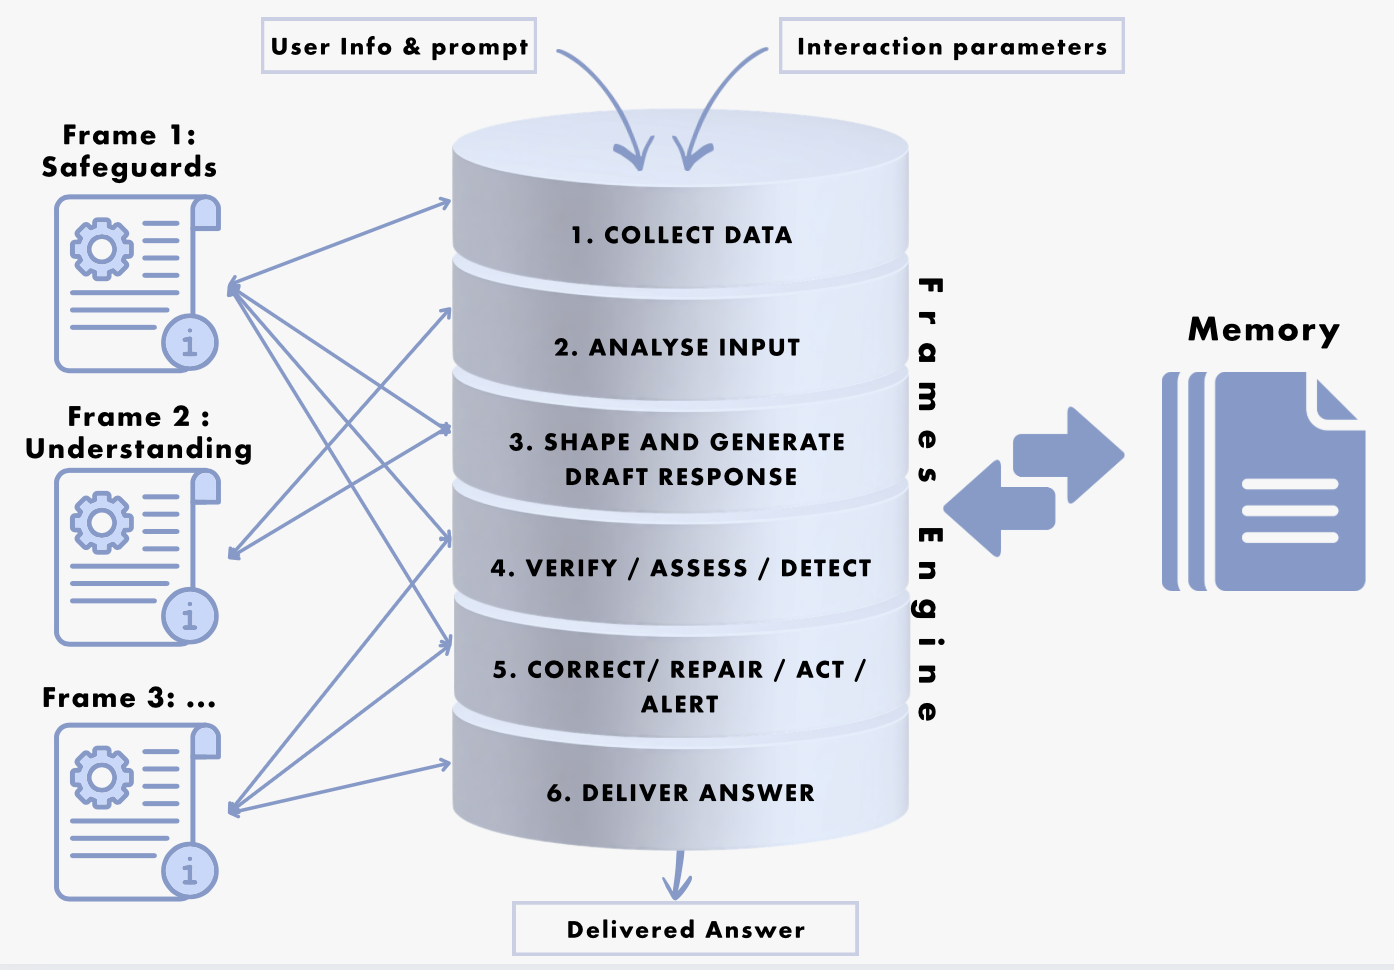
\includegraphics[width=0.7\linewidth]{Images for manuscript/Figure 3}
\caption{Illustration of the SCAFFOLD structure}
\label{fig:scaffold}
\end{figure}

The SCAFFOLD framework proposes a modular system of frames as illustrated in \textbf{Figure 3}. We define a frame as a coded layer between the user and the LLM that handles a set of tasks, such as a system of checks at different stages of the process. A frame could work with different LLMs and in different contexts and it communicates with a memory. The frames are compiled in a frame engine, the core of the system, which follows several steps:

\textbf{1: Collect data.} This step collects the information from the user, such as age, nickname, location, prompt; from the parameters of the designed interaction, such as what checks to run, what is the goal of the interaction, etc.; from memory, such as the conversation logs, previous checks results, etc. This first step feeds the others.

\textbf{2: Analyse input.} This second step allows to assess different levels of risks and trigger safety measures that are difficult to put in place otherwise. For example, sending an alert to a teacher when a student insists at misusing the tool or when a student is expressing dark thoughts, but also to trigger meta-responses when the user goes off topic. Another advantage of an input analysis is to be able to assess users' cognitive and emotional engagement, an aspect that is particularly relevant in educational settings. Moreover, input analysis allows to perform analysis that can be used to improve the interaction in real time or to analyse the interaction afterwards. Examples of analyses can be the user's understanding of the content, progress towards a goal, their level of critical thinking, level of engagement or fatigue. Some analyses can be quite simple and straightforward, such as the level of distraction from the topic, while other analyses could be more complex and require expert validation, such as in the case of detecting learning difficulties or mental health problems.

\textbf{3: Shape and generate draft response.} Step 3 consists of shaping the prompt in a way to take into account (1) a constitution which integrates safeguards as prompts, (2) the context of the interaction -- parametrization -- with information from parametrization of the interaction and user information, (3) the results of the input analysis, and the (4) user's prompt and information from memory such as conversation logs. This step also includes the generation of a drafted response by an LLM. When the model is used in real time interactions, processing speed might become a crucial factor in deciding which model to use, while for offline analysis or when the interaction is only monitored, a more heavy, slow model might be more appropriate.

\textbf{4. Verify / assess / detect.} Step 4 runs validation checks on the generated draft, such as verifying the alignment with safeguards and the parametrization of the interaction. Additional analyses could be added for specific checks such as for biases, cultural pertinence, or accuracy.

\textbf{5. Correct/ repair / act / alert.} Step 5 considers the results of the previous checks to decide the subsequent actions. For example, if the safeguards checks are not passed, it can trigger a correct--reverify loop (i.e.,a repair procedure). This loop regenerates an answer adding more specific instructions to the prompt and rechecking that answer until it either passes the checks or reaches a maximum number of repairs. When the limit of repairs is reached a fallback or a notification to a responsible adult can be triggered. Ideally the correct-verify loop is a non-regression safeguard (i.e., does not re-introduce an error that was already fixed). If a repair regresses, or if the budget (iterations and time) is exhausted, the system should return a pre-approved safe fallback. The correct-reverify loop can be bypassed in certain cases (e.g. a technical problem or a red flag), In this case, it would be possible to use a shortcut to a fallout. A fallout can be asking the student to contact an adult, generating an alert or triggering reports.

\textbf{6. Deliver Answer.} Step 6 states the final answer to deliver to the user in that turn and saves it to the memory.

It is useful to distinguish the two types of checks that are used in the framework: \textbf{deterministic checks} enforce rules that can be written in code, such as interaction time monitoring, or user's turn counting. \textbf{Probabilistic checks} use queries to a lighter or a specialized LLM, called LLM‑as‑a‑judge or AI judges \cite{Baysan2025, Gu2026} that can evaluate semantic and pedagogical properties, for example whether the question is on topic. These AI judges will need appropriate validations and reliability checks before deployment. Potentially a multi-agent evaluation method could be used to increase reliability and consistency, though it might be insufficiently quick for real-time conversations.

SCAFFOLD needs an \textbf{external memory} to run effectively. The memory is needed at conversation level and can be re-initiated at each new interaction, leaving no traces. It is also possible to have a memory that tracks multiple conversations which can be useful in assessments, evaluation or personalization of the content, monitoring long-term progress of students, and tracking the content covered. Monitoring can have positive impacts such as teachers' changing their time allocation towards students that are more in need \cite{Holstein2018} and fostering pro-social behavior \cite{Canigueral2019}. However, monitoring can also be negatively perceived by the students if it is imposed and/or they are not aware of it, potentially increasing anxiety \cite{Canigueral2019}. It is crucial therefore to limit monitoring to when there are clear benefits for educators and students. An implementation of the framework should therefore aim at transparent practices about what is being monitored, how, and who has access to that information. Users should be able to activate or deactivate memory preservation after the interaction.

\section*{3. Pilot study: Application of SCAFFOLD in a school setting}

To explore and validate the practical deployability, efficacy and interest of SCAFFOLD, we designed a minimal SCAFFOLD framework which we piloted in two classes with children between 12 to 16 years. Our main goal was to explore the feasibility and usefulness of deploying SCAFFOLD in an educational setting. We additionally preregistered the following research questions:

\begin{itemize}
\item RQ1: To what extent can SCAFFOLD support children's short-term and long-term learning?
\item RQ2: How accurately can SCAFFOLD assess children's understanding?
\item RQ3: To what extent can SCAFFOLD balance students' contributions in a group?
\item RQ4: Is children's co-creation with SCAFFOLD predicted by their prior knowledge*?
\end{itemize}

\subsection*{3.1 Methods and materials}

\subsubsection*{3.1.1 Participants}

We recruited two classes from a rural German comprehensive school, consisting of 27 children (M = 13.46 years, SD = 0.81, 4 female, 21 male, 2 other/not specified) and two teachers (M = 45.50, SD = 4.95, 2 female). For a technical reason, we lost the LLM interaction data of one group and therefore report findings of 24 students and nine groups. Participants were German native speakers and provided written (parental) consent. The experiment was approved by the local ethics committee (25 ETHICS-247).

\subsubsection*{3.1.2 Robot and Interface}

The students interacted with the LLM through a custom computer interface and a robot called Marty, both developed by Robotical ltd. Marty robot is a medium-sized, educational humanoid robot, with movement and speech capabilities, designed to support STEAM education. Designed for learners as young as 4 to support programming learning \cite{Robotical2024}, Marty robot was chosen for several reasons related to a parallel project involving building of the robot, programming it, and interacting with it. A custom web interface was deployed for this study, based on the standard Robotical web application. The interface was modified to integrate the SCAFFOLD pedagogical framework and support the experimental design requirements. More details are available in the S4.

\subsubsection*{3.1.3 Description of Marty's SCAFFOLD design}

Students-AI interaction consisted in co-creating a mnemonic, such as a story, a poem or a few jokes, in groups of 2 to 3 students on a topic previously covered in class. Mnemonics are memory-aiding techniques used to improve long-term memorisation and recall building on cues, concreteness, associations, and/or other types of connections and has been chosen for its potential to increase learning \cite{Clark1991, Fung2024}. Marty's SCAFFOLD design was set to last 10 minutes and follow three phases: (i) First, students were prompted to select the microcontrollers concepts to include in the mnemonic; (ii) in the second phase, students co-create the mnemonic with Marty; and (iii) in the third phase students should memorize the mnemonic. The parametrization of the interaction is described in \textbf{Figure 5}. Because the initially set time was too little, groups did not reach the third phase.

We developed the general architecture to run the six SCAFFOLD stages (collect data, analyse input, shape and generate draft response, verify, repair and deliver answer; see \textbf{Figure 3};S1). While this architecture can run on any LLM model, we used gpt-4.1-mini on Microsoft Azure for this pilot. Since the interaction involved the social robot Marty, we additionally deployed text to speech and speech to text by using a Microsoft Azure male standard voice.

\begin{figure}[htbp]
\centering
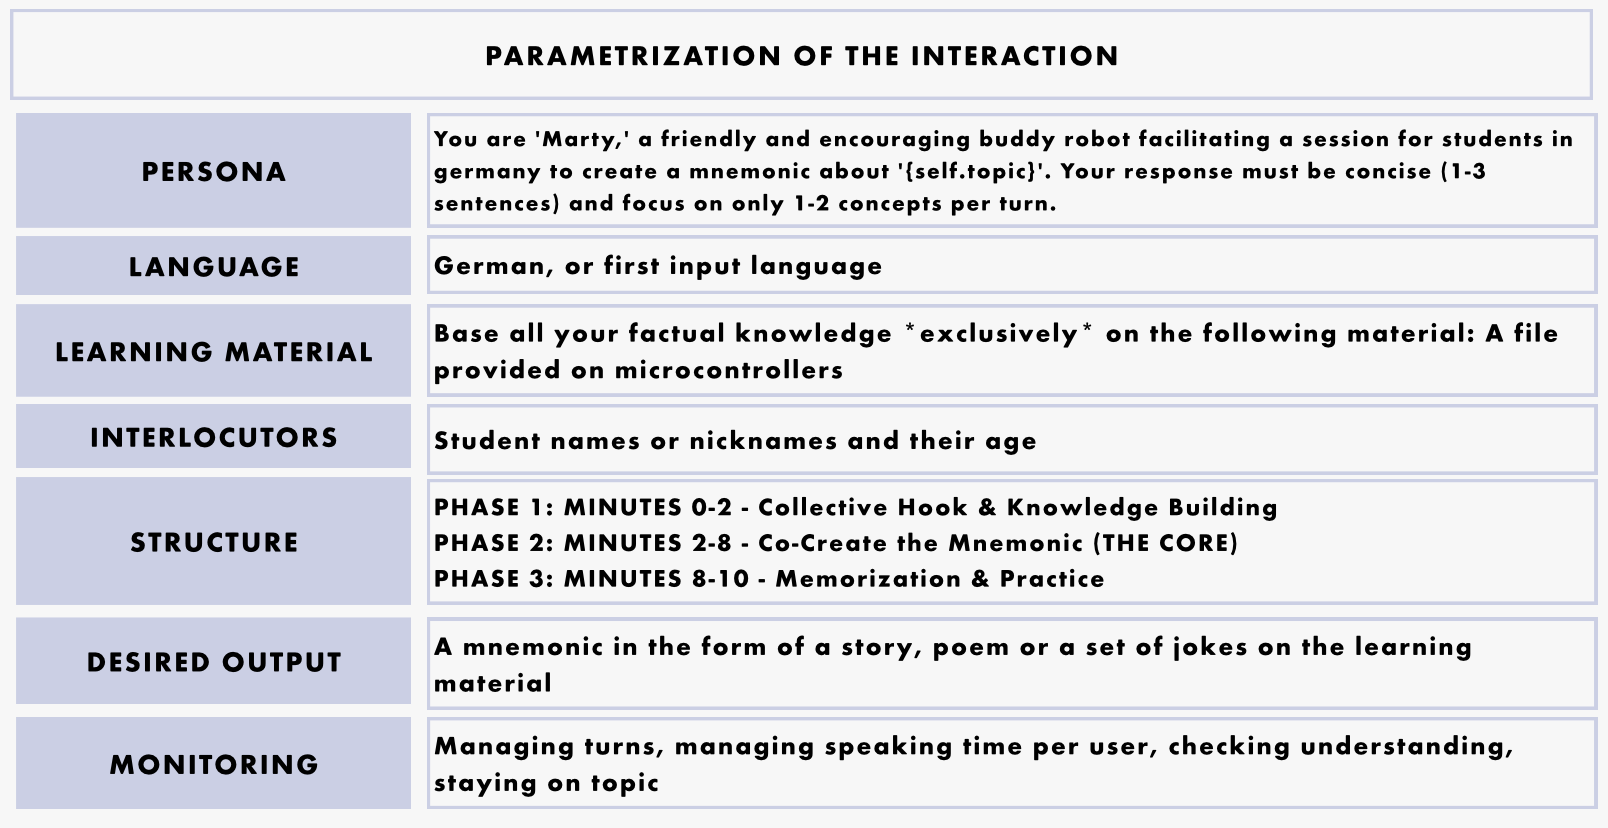
\includegraphics[width=\linewidth]{Images for manuscript/Figure 5}
\caption{Marty's interaction parameters}
\label{fig:marty-params}
\end{figure}

We created five frames implemented throughout the six stages of the frame engine and detailed in Table 1: the main frame ``Mnemonic CoCreator Frame'' (1), which managed most of the checks, and four more specific validation frames. The ``language checker'' frame (2) assessed age appropriate language, tone, and complexity of responses. The ``balanced turns'' frame (3) managed fair turn-taking across students, tracking participation count, speaking time, and consecutive turns. The ``comprehension tracker'' frame (4) maintained per-student, per-concept understanding profiles, tracking whether each student understands, is confused about, or has misconceptions regarding specific concepts. Lastly, the ``phase checker'' frame (5) ensured that responses aligned with the current session phase goals and pedagogical requirements (see supplementary material S2 for more details).

\begin{table}[htbp]
\centering
\begin{tabular}{|l|p{5cm}|p{5cm}|}
\hline
\textbf{Frame} & \textbf{Responsibility} & \textbf{Key Checks} \\
\hline
Mnemonic CoCreator & Session management, phase transitions, mnemonic building & Time-based phases, contribution analysis, mnemonic quality \\
\hline
Language Checker & Age-appropriate language & Complexity, tone, technical terms usage \\
\hline
Balanced Turns & Fair participation & Turn counts, speaking time, monopolization detection \\
\hline
Comprehension Tracker & Understanding monitoring & Per-student, per-concept profiles \\
\hline
Phase Checker & Phase alignment & Phase-specific goals and pedagogical requirements \\
\hline
\end{tabular}
\caption{\label{tbl:frames}Overview of frames with their responsibility and key checks}
\end{table}

The frames communicated via a \texttt{shared\_context} dictionary for ephemeral data within a turn and a \texttt{frame\_memory} dictionary for persistent state across turns. Prior to the pilot deployment, the framework was tested in 3 ways: (i) manually, (ii) with static simulations, and (iii) with dynamic simulations using three student personas impersonated by another LLM (see supplementary material S3 for more details).

\subsubsection*{3.1.4 Procedure}

The pilot was conducted as part of an experimental study (Leisten et al, in prep.), in which students participated in a 7-weeks AI literacy training centered around building and interacting with the social robot Marty \cite{Robotical2024}. The curriculum covered topics such as AI, LLMs, social robots, programming, sensors, and microcontrollers. We deployed the SCAFFOLD framework in the last session of the 7-weeks curriculum in which students worked in randomly assigned groups of 3-4 to create a mnemonic (a poem, a story or a few jokes) about microcontrollers with the support of Marty. A summary of the microcontrollers learning materials covered in class was provided both to students and the LLM. First, students created a mnemonic using the LLM out of the box. Students then created a second mnemonic with the SCAFFOLD framework enabled. Each mnemonic session lasted approximately 10-15 minutes.

We administered pre-, post-, and feedback surveys in Qualtrics \cite{Qualtrics2024} to students at several timepoints during the 7-weeks curriculum. Here, we report the results relevant for the evaluation of SCAFFOLD, specifically children's knowledge about microcontrollers, assessed in the pre-test (conducted at week 1; T1), post-test (conducted at week 7; T2), and the learning retention test (conducted 7 weeks after T2; T3), as well as students' and teachers' feedback about the LLM interactions. All code and data are available on \href{https://github.com/OlgaMuss/LLM_Frames_Paper}{github} and a simulation app on \href{https://buildbot-4tzkvoxzssupnzkb9e6va4.streamlit.app}{streamlit cloud}. More detail on the methodology can be found in the Supplementary Materials S4.

Student speech was captured by the computer's microphone and transmitted to Microsoft Azure for speech-to-text transcription, LLM inference (gpt-4.1-mini), and text-to-speech synthesis.

\begin{figure}[htbp]
\centering
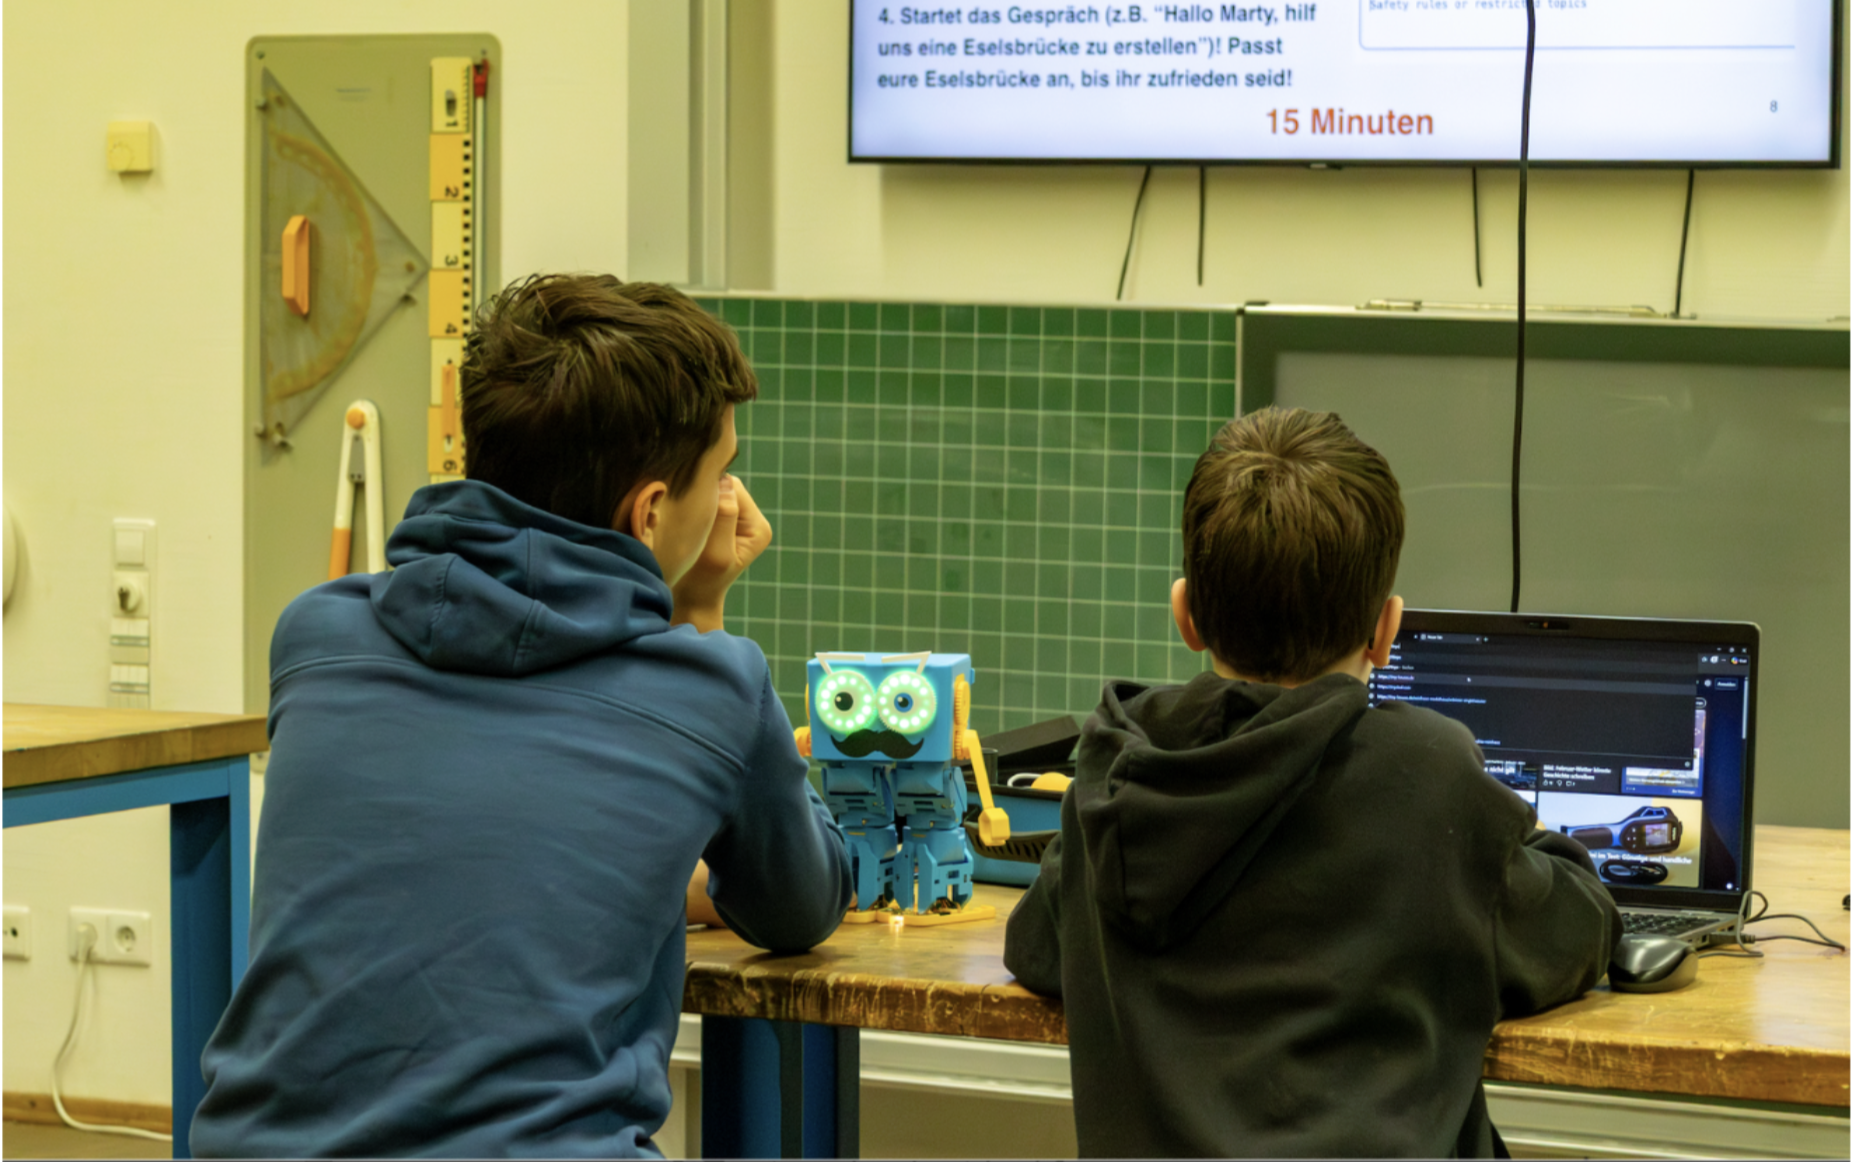
\includegraphics[width=0.8\linewidth]{Images for manuscript/Figure 4}
\caption{Illustration of the setting of the interaction}
\label{fig:setting}
\end{figure}

\subsubsection*{3.1.5 Measurements}

\textbf{Students' microcontroller knowledge.} We assessed students' microcontroller knowledge at T1 with two questions and added another eight questions at T2 and T3, based on the learning materials covered in class (see Supplementary Materials S4 for items). The single-choice questions covered what a microcontroller is, its function, components, and a few technical details (voltage, pins, programming language). Children were instructed to select one out of five answer options (one of them being ``\textit{I don't know}'') for each item, resulting in a possible score of 0-2 at T1, and 0-10 at T2/T3 (1 = correct, 0 = wrong, 99 = don't know, later coded as 0 for main analyses).

\textbf{Students' perception.} We assessed students' intrinsic motivation after the session using a shortened and adapted version of the intrinsic motivation inventory \cite{Deci1985, Wilde2009}, previously used by \cite{Heindl2020} and \cite{Rollke2022} in children's samples. In eight items, students' indicated their perceived enjoyment, competence, tension, and usefulness of the class activities on a 5-point Likert scale (1 = does not apply, 5 = applies fully). Additionally, we added five questions specific to the LLM interaction, in which we asked about enjoyment, perceived learning gains, and equal contribution of team members on a 5-point Likert scale (1 = very bad / very little / not at all, 5 = very good / very much / absolutely), and two open-ended questions for positive and negative feedback.

\textbf{Teachers' perception.} Teachers completed a feedback survey after the session, including 12 quantitative questions assessing perceived student engagement and learning, difficulty, and items specific to the LLM interaction (e.g., helpfulness, difficulty, entertaining). Additionally, teachers provided open-ended positive and negative feedback.

\textbf{LLM interaction measures.} We collected Marty's interaction logs to analyse students' interactions with the LLM. These logs included session IDs, timestamps, LLM instructions, user and system prompts, turns, and students nicknames. The SCAFFOLD logs additionally included the frames meta data as described below. The students' interaction logs were analysed manually, describing each turn and coding when students proposed ideas or concepts relevant to the mnemonic.

\textit{Contributions and off-topic turns}

Each student prompt was manually coded for being on or off topic, a concept to include in the mnemonic and which concept, and constructive for the creation of the mnemonic or not.

\textit{Balanced turns}

For each conversation, we coded the number of turns each student spoke, and then used the Gini coefficient to estimate equity of turns. The Gini coefficient \cite{Dixon1987} is a statistical measure of inequality in a distribution, most commonly used to measure income or wealth inequality within a population.

\textit{Co-creation level}

While we pre-registered the length and depth of the created mnemonic as an indicator of learning success, we later realized that the mnemonic was sometimes created by the LLM and therefore did not represent students' engagement or contribution. We therefore decided to use another variable that we defined at the pre-registration: the co-creation level ( ``0: LLM did it all, 1: concepts by kids/rest LLM, 2: concepts by the students, co-creation of the mnemonic, 3: mainly by students). This variable was coded manually by two raters using a decision tree available in S4. The coding was done per group counting students' contributions to each phase and considering the depth of the contribution (e.g. one very simple concept vs. several complex ones). We added a 0.5 level a posteriori to integrate the case where students contributed in guiding the LLM, but did not contribute to the concepts.

\subsubsection*{3.1.6 Data analysis}

Statistical analyses were performed in R \cite{RCore2020} using RStudio \cite{Posit2025} and Python (version 3.12.12; \cite{Python2021}) using Jupyter Notebooks \cite{Kluyver2016}. Since the aim of this pilot was to test the feasibility and potential benefits of SCAFFOLD, statistical analyses are mainly descriptive. Co-creation level coding inter-rater reliability was assessed using Cohen's $\kappa$ (unweighted and weighted) and Pearson's \textit{r}. Weighted $\kappa$ is reported as the primary measure due to the ordinal nature of the scale \cite{Landis1977}. To answer RQ1 and RQ4, we fit a linear mixed-effects model with children's post-test knowledge scores (T2: immediate post-test; T3: delayed post-test) as the outcome variable, co-creation level, timepoint (immediate vs. delayed), and prior knowledge (T1) as fixed effects, and participant as a random effects to account for repeated measures. We fit a linear mixed-effects model using the lmer() function from the lme4 package \cite{Bates2015} with p-values computed using the lmerTest package \cite{Kuznetsova2017}. We originally preregistered separate linear mixed effects models per timepoint, which we ran and their results are available in supplementary material S5. However a combined model allows to account for the nested nature of the data and to control for prior knowledge and therefore has been chosen for reporting.

\subsection*{3.2 Results}

The aim of this pilot was to test the feasibility, usability, and utility of the frame for supporting children's learning. We successfully implemented the framework, enabling students to co-create a mnemonic with a social robot, highlighting the feasibility and usability. Below, we report the findings organized by relevance, including both descriptive findings and preregistered analyses.

\begin{figure}[htbp]
\centering
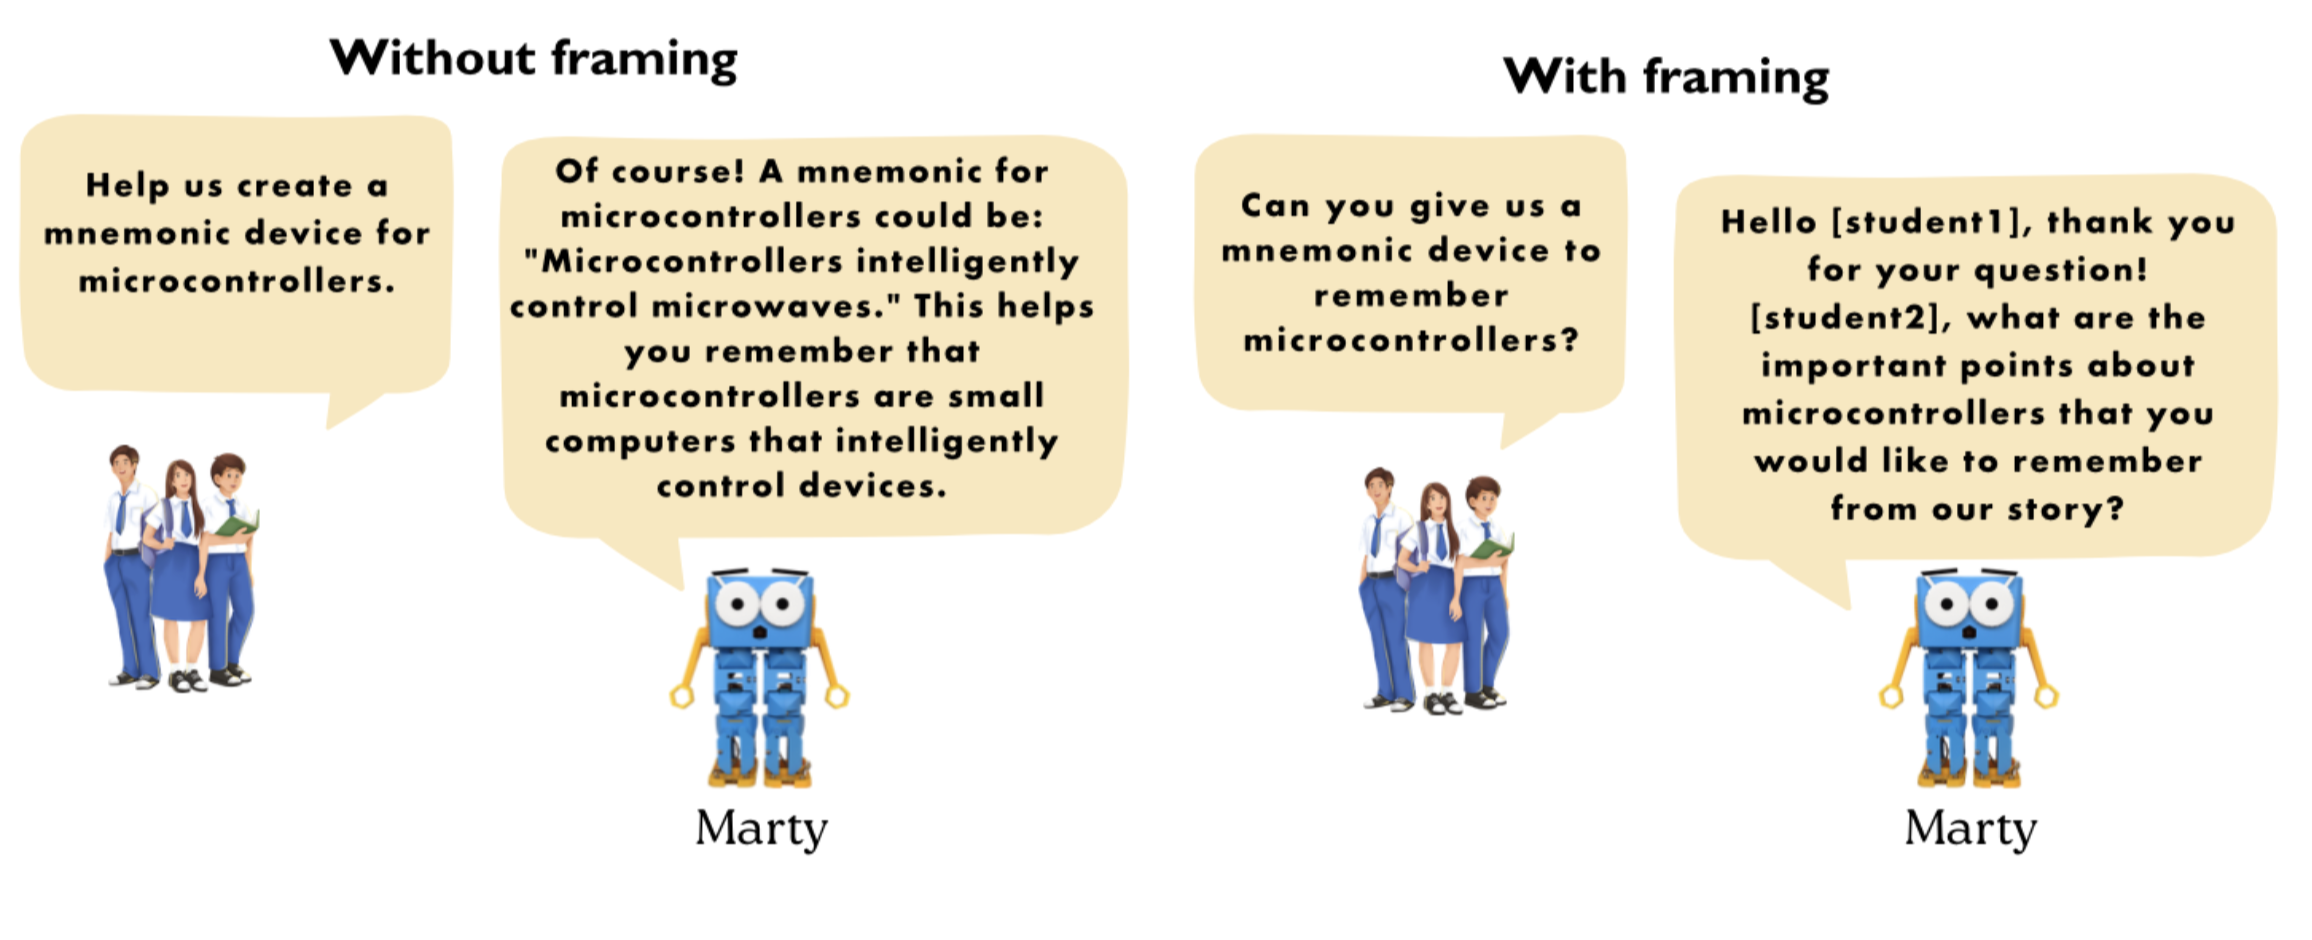
\includegraphics[width=\linewidth]{Images for manuscript/Figure 6}
\caption{Example of answers without and with SCAFFOLD framing}
\label{fig:comparison}
\end{figure}

\subsubsection*{Finding 1 : Students were more active with SCAFFOLD than without}

The main impact of the SCAFFOLD frame was that students contributed to the creation of the mnemonic, a behavior that was absent from their LLM interactions without SCAFFOLD. Students contributed to the identification of concepts to include in the mnemonic (18 relevant suggestions by 13/24 students) and to the actual creation of the mnemonic (13 suggestions from 12/24 students, \textbf{Figure 7}). This is an important shift from students being mere consumers of AI technology to becoming active creators.

\begin{figure}[htbp]
\centering
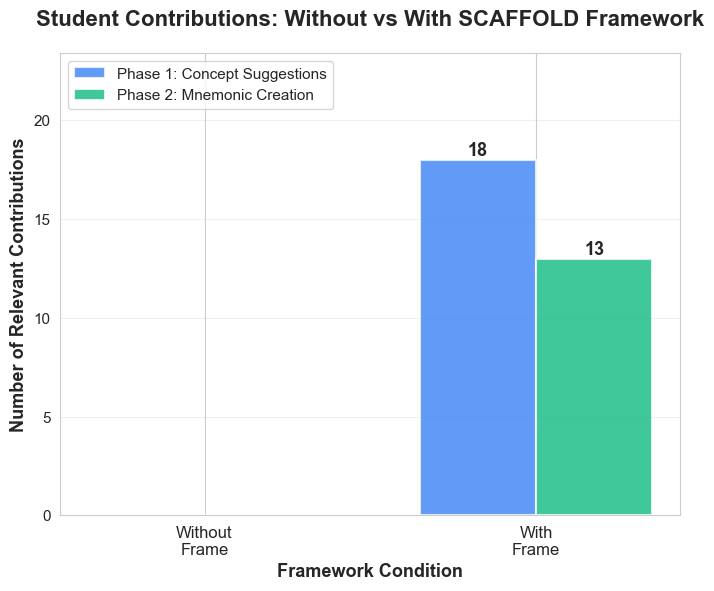
\includegraphics[width=0.7\linewidth]{Images for manuscript/Figure 7 contributions}
\caption{Students' contributions per phase with and without the SCAFFOLD framework}
\label{fig:contributions}
\end{figure}

While all groups successfully created a mnemonic, two groups fully co-created it, two groups provided the concepts with the LLM proposing a mnemonic, and one group provided input for the creation of the mnemonic. The remaining four groups provided only limited input to the mnemonic creation.

\subsubsection*{Finding 2: SCAFFOLD supports more balanced turn taking (RQ3)}

Another important aspect was a more balanced involvement of students (RQ3). Without SCAFFOLD, six students did not participate in the interaction at all, while only one student did not participate in the interaction with SCAFFOLD. While participation was not significantly more equitable (\textit{W = 9.00}, \textit{p} = .13), the balance between turns was more reliable (i.e., varied less; \textit{F} = 5.84, \textit{p} = .02); \textbf{Figure 8}). From this exploratory analysis, the balanced turns frame appears to have worked well and succeeded in guiding a more balanced interaction, setting an example for multi-user interactions with AI.

\begin{figure}[htbp]
\centering
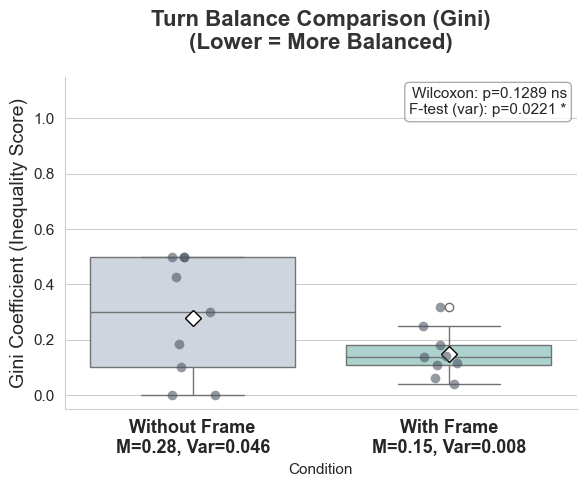
\includegraphics[width=0.65\linewidth]{Images for manuscript/Figure 8 gini}
\caption{Gini Coefficient \cite{Dixon1987} assessing the level of equitable participation in interaction without or with SCAFFOLD framing. The dots represent Gini coefficients per group.}
\label{fig:gini}
\end{figure}

\subsubsection*{Finding 3: Higher co-creation level was associated with higher post-test knowledge scores and not predicted by prior knowledge (RQ1 \& RQ4)}

Children's post-test microcontroller knowledge was significantly associated with their co-creation level (\textit{b} = 1.06, \textit{SE} = 0.35, \textit{p} = .005; \textbf{Figure 9}), indicating that higher student engagement during mnemonic creation was associated with better learning outcomes. This effect remained significant when controlling for prior knowledge (T1), which itself did not predict post-test scores (\textit{b} = -0.13, \textit{SE} = 0.49, \textit{p} = .79; \textbf{Figure 9}). There was no significant main effect of timepoint (\textit{b} = -0.09, \textit{SE} = 0.63, \textit{p} = .88), suggesting similar overall performance on immediate (T2) and delayed (T3) post-tests. The co-creation and timepoint interaction was not significant (\textit{b} = -0.59, \textit{SE} = 0.38, \textit{p} = .13). Co-creation level coding inter-rater reliability was almost perfect (weighted $\kappa$ = 0.82, 95\% CI [0.70, 0.95]), with 44.4\% exact agreement (4/9 groups). Unweighted $\kappa$ = 0.35 (95\% CI [0.03, 0.66], fair) and Pearson's \textit{r} = 0.894 (\textit{p} = .001). The five disagreements were resolved through discussion between raters.

\begin{figure}[htbp]
\centering
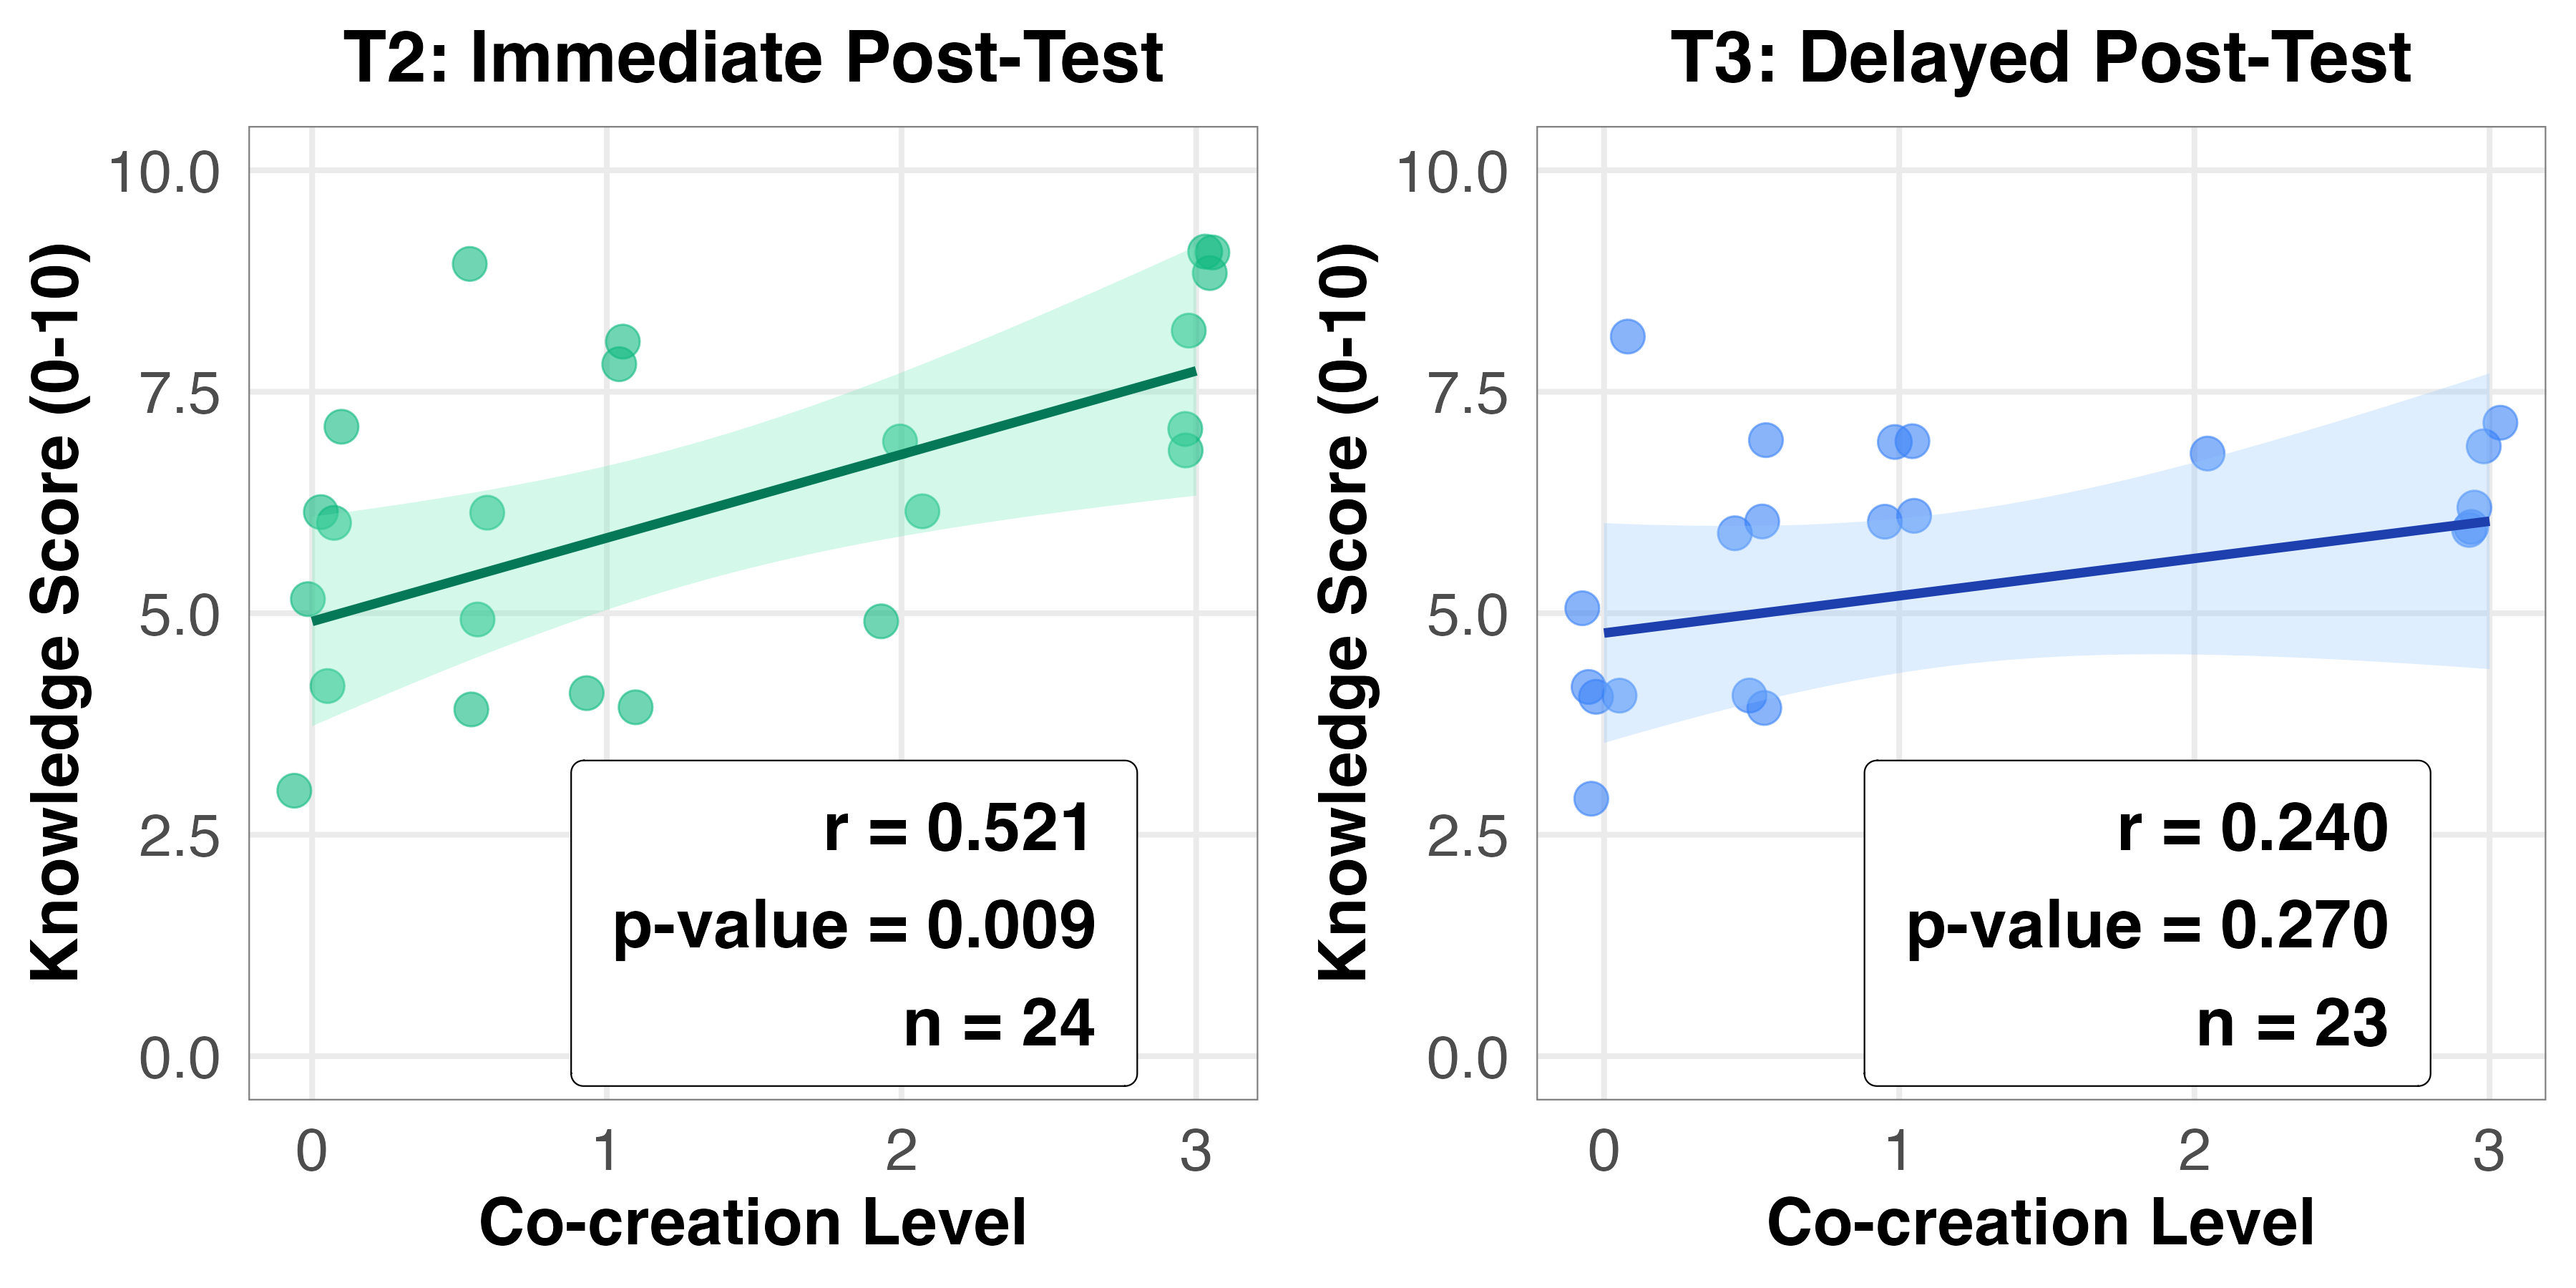
\includegraphics[width=0.8\linewidth]{Images for manuscript/Figure 9 T2 and T3}
\caption{Association between co-creation level and microcontrollers knowledge at posttest (T2) and learning retention test (T3). Co-creation level defined as: 0: LLM did it all, 0.5: some guidance from students unrelated to learning, 1: concepts by students/rest LLM, 2: concepts by the students, co-creation of the mnemonic, 3: mainly by students).}
\label{fig:correlation}
\end{figure}

\subsubsection*{Finding 4: SCAFFOLD reduces off-topic turns}

Students' off-topic turns decreased from 38\% without the framing to 1\% with SCAFFOLD (\textit{W} = 0.00, \textit{p} = .03; \textbf{Figure 10}). This suggests that students were more engaged in the activity, potentially because Marty was asking individual students directly.

\begin{figure}[htbp]
\centering
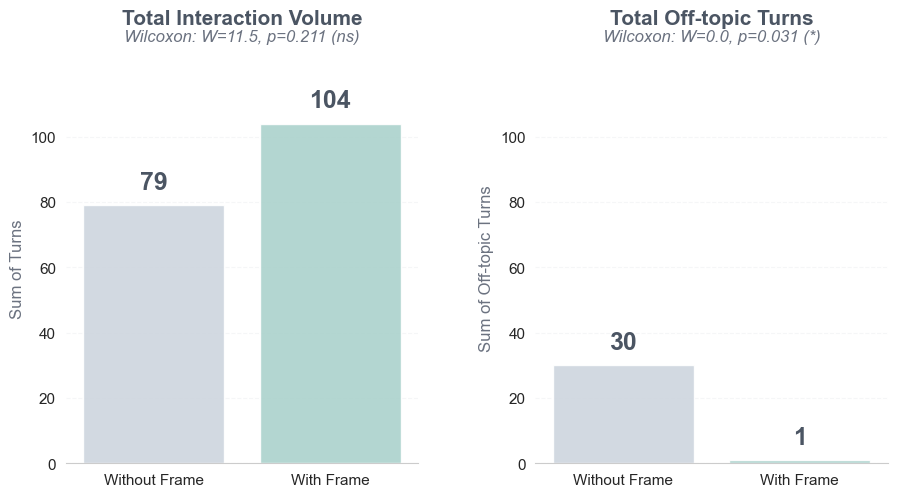
\includegraphics[width=0.6\linewidth]{Images for manuscript/Figure 10 off topic}
\caption{Total number of turns in general and turns off-topic without and with SCAFFOLD framing}
\label{fig:offtopic}
\end{figure}

\subsubsection*{Finding 5: Students and teachers enjoyed the activity}

In general students rather enjoyed the activity (\textit{M} = 3.96, \textit{SD} = 0.92) and thought that the LLM interaction has helped them learn (\textit{M} = 3.27, \textit{SD} = 1.12, \textbf{Figure 12}), with several students reporting creation as a mnemonic with Marty as what they liked about the LLM interaction with SCAFFOLD. Negative feedback came mainly from groups that ran out of time, which resulted in Marty resisting to answer and instead indicating that their time was over. Both teachers also considered the activity helpful (\textit{M} = 3, \textit{SD} = 0) and somewhat engaging (\textit{M} = 4, \textit{SD} = 0).

\begin{figure}[htbp]
\centering
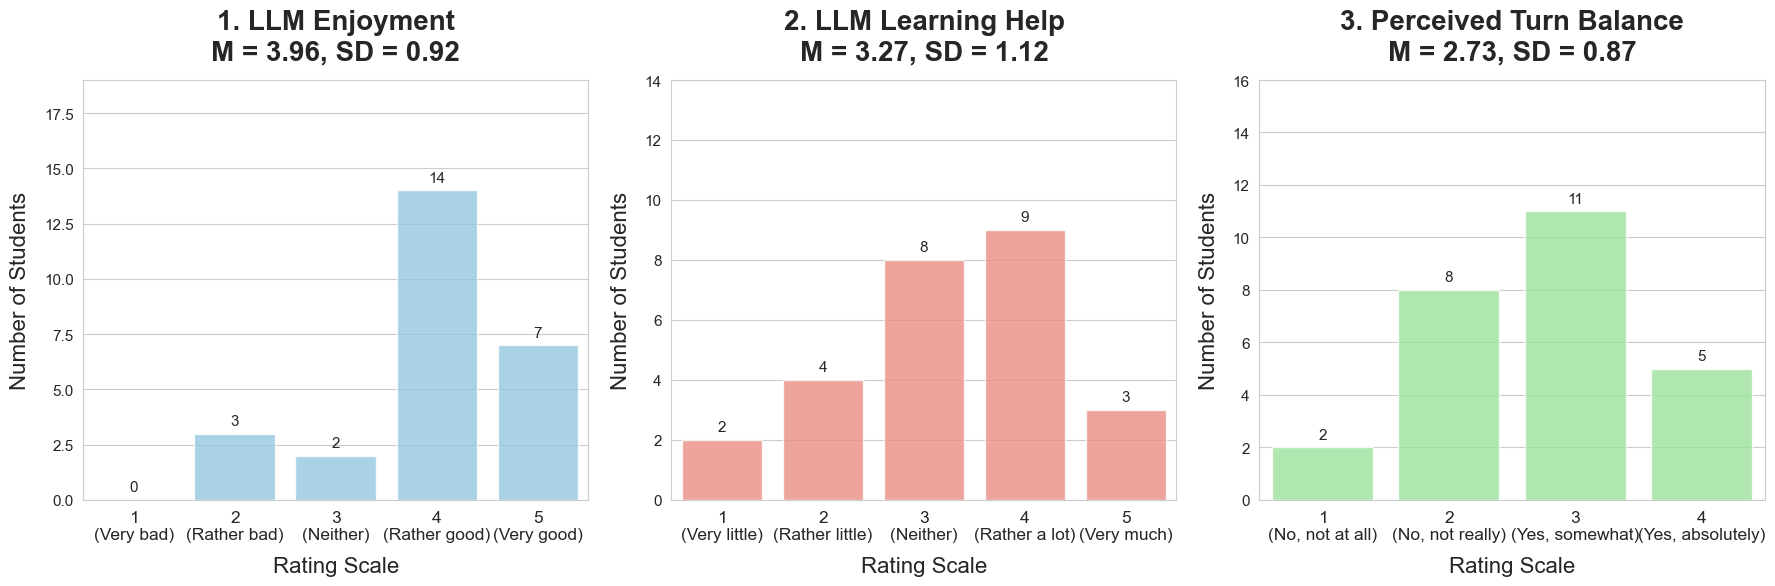
\includegraphics[width=\linewidth]{Images for manuscript/Figure 12}
\caption{Students feedback on the interaction with Marty using SCAFFOLD: 1. LLM enjoyment: How did you like your last voice interaction with Marty? (1-5), 2. LLM Learning Help: How much did your last conversation with Marty help you learn? (1-5), 3. Perceived Turn Balance: Did you feel everyone talked to Marty equally? (1-4)}
\label{fig:feedback}
\end{figure}

\subsubsection*{Finding 6: Scaffold was not able to assess understanding}

Our research question RQ2 was: ``\textit{To what extent did the frame accurately assess children's understanding?}'' and we observe that our setting of the framing failed to accurately assess understanding, as we see from manual assessment of the frame's logs. In part, this is due to the very little input from the students, in part because we haven't defined well enough how the statistical checker should assess understanding. This topic is very complex and would benefit from further research.

Overall, the pilot showed potential for engagement and learning, and while the developed framework is far from perfect, it was an improvement from the standard LLM interaction without framing.

\section*{4. Discussion}

In this paper, we present SCAFFOLD, a methodology that supports the implementation of safer and more beneficial LLM interactions in educational settings. SCAFFOLD is designed to be model-agnostic, allowing the open-source community to develop an ecosystem of safeguards and pedagogical behaviours in collaboration with educators and child development experts. The methodology enables AI integration in education that goes beyond individual screen-based interaction, towards dynamic, social learning potentially supported by multi-user AI interactions or by assisting teachers in analysing conversations with or between students. The modularity and control over data storage and processing, enabling privacy-preserving deployment when paired with local infrastructure, is a further advantage, allowing schools to minimise data sharing while delivering the benefits of personalisation and differentiation.

We piloted SCAFFOLD in a short multi-user interaction in a classroom setting with 12-16-year-olds, demonstrating feasibility and a potential for supporting learning and engagement. Students were more engaged with the framed AI, proposing concepts and ideas, a behavior absent without the framing. With the framed LLM, students stayed on topic more. While the reasons behind this increased on-topic contributions would need to be further investigated, it seems natural that once the LLM provided the mnemonic for the students they tended to move to a new exploration, while a framed LLM, instructed to redirect if someone goes of topic, which happened once, helped students to stay on the task.

Students' turn-taking was more reliable, probably because the LLM directed questions at individual students using their nicknames, even if they did not always respect this guidance. It is important to note that, ideally, an interaction would imply minimal input from an AI, with students working out the mnemonic as autonomously as possible. This would mean that several students might speak one after another, with no intervention from the LLM. While this is possible in general -- we tested that in the prototype version -- we were not able to implement it due to time constraints. Since our analysis did not take into account the turns of the LLM itself further research should explore how allowing users to speak one after another with the AI intervening only when needed, could balance speaking time not only between students but also between students and AI.

Students that contributed more to the mnemonic creation, such as a poem or a story to better remember concepts covered in class, also had higher post-test scores, suggesting that SCAFFOLD could have a potential to support learning. While we did not expect to see these positive results in such a short exercise, the findings are consistent with the retrieval practice in the literature \cite{Roediger2011}: remembering strengthens retention. Contributing more to the creation of the mnemonic may have helped students to remember the learning content and consequently helped them retrieve the knowledge later. More future research is needed to formally evaluate the potential of a framed LLM to support learning.

Our findings resonate with a broader principle: in the age of generative AI, producing content is effortless, but learning requires effort. SCAFFOLD is designed to preserve that productive effort, supporting ``human-AI co-thinking'' \cite{BardynForthcoming}. Keeping students, and educators, at the centre of the interaction, not as consumers of AI output, but directing, verifying, and shaping the collaboration. While the framework provides the technical infrastructure for this mode of interaction, deciding what students should learn remains a profoundly human responsibility.

The exploratory nature of our pilot comes with several limitations. First, SCAFFOLD failed to accurately assess students' understanding (RQ2). In part, this is due to the little input from the students because of the short time they had per person, and in part because we did not define well enough how the probabilistic checker should assess understanding. Second, the interaction time was set too short to reach the third phase when the students were supposed to practice the mnemonic. While the closure worked well at first, we did not define what should happen if the students kept interacting with Marty. Also all groups interacted first with no frame, with no counterbalancing for pedagogical reasons. While we would expect less engagement with the second task due to fatigue and novelty wearing up, this would need to be confirmed.

In the future, it would be useful to add a strong cutoff when the interaction stops completely or provide more guidance to students what to do when the LLM tries to stop the interaction. Also, some students indicated that they would have liked to explore other topics with Marty, indicating that we should have added an exploration session before jumping into a structured interaction. Finally, we sampled a small, homogenous sample limiting the generalizability of our results.

Future work should extend and go beyond the piloted frame, which was a first step towards a usable version, and involve educators and experts in the design, test and iterative improvement of students-AI interactions. For example, the balanced turns frame was reliably successful in its task to ensure balanced turns between students and needs further testing, while the comprehension checker frame needs to be developed to include multi-dimentionality of learning and empirical validation of the accuracy of the probabilistic checks. Our results point to a potential for further research: a research that is crucial when the largest proportion of those using LLMs are teenagers, often without proper training and safeguards from the service providers or regulators.

\section*{Acknowledgements}

We thank the participating school, the teachers who facilitated the classroom sessions, the students who participated in the study, and the Robotical Ltd team for their technical support.

\section*{Competing interests}

Partial funding was received by the Social Brain Sciences Lab.

\section*{Data availability statement}

All data supporting the findings of this study are openly available in the GitHub repository at \href{https://github.com/OlgaMuss/LLM_Frames_Paper}{https://github.com/OlgaMuss/LLM\_Frames\_Paper}. The repository includes:

\begin{itemize}
\item Student knowledge assessment data (anonymized with participant IDs)
\item Student and teacher feedback survey data
\item LLM interaction transcripts (with pseudonyms)
\item Manually coded behavioral analysis data
\item Complete codebook for all measures
\item All analysis code (Python and R)
\item Supplementary materials (S1-S9)
\end{itemize}

An interactive simulation app demonstrating the SCAFFOLD framework is available at \href{https://buildbot-4tzkvoxzssupnzkb9e6va4.streamlit.app}{https://buildbot-4tzkvoxzssupnzkb9e6va4.streamlit.app}. The study preregistration is available at \href{https://doi.org/10.17605/OSF.IO/K7UE2}{https://doi.org/10.17605/OSF.IO/K7UE2}.

\bibliography{references}

\section*{Annexes}

\subsection*{Supplementary materials}

\begin{itemize}
\item S1: Framework Architecture
\item S2: Frame implementation
\item S3: Testing
\item S4: Classroom pilot methods
\item S5: Pilot statistical analysis
\item S6: Learning material
\item S7: Codebook for qualtrics
\item S8: \href{https://docs.google.com/document/d/1H8ze6IJ8H7I5qsTjTcrK8b4FXwIk0rf9yr8sr4EKXkY/edit?tab=t.0}{Detailed LLM Interaction notes}
\item S9: \href{https://github.com/OlgaMuss/LLM_Frames_Paper/blob/main/Data_analysis/Data/BuildbotAnalysis\%20-\%20LLM\%20analysis.csv}{LLM interaction coding and co-creation level calculation}
\end{itemize}


\subsection*{Other links}

\begin{itemize}
\item \href{https://github.com/OlgaMuss/LLM_Frames_Paper}{github}
\item simulation app on \href{https://buildbot-4tzkvoxzssupnzkb9e6va4.streamlit.app}{streamlit cloud}
\item pre-registeration: 10.17605/\href{http://OSF.IO/K7UE2}{OSF.IO/K7UE2}
\end{itemize}

\subsection*{Statement on GenAI use}

\begin{itemize}
\item This paper has been written without the help of an AI. After writing, Gemini was used for proofreading.
\item We used Cursor with several models for fine-tuning and debugging the frame's code.
\item We used Claude for a first draft of the supplementary materials S1, S2 and S3 generation based on the existing code, which we reviewed and adjusted afterwards.
\item We used Cursor to assist in writing data analysis code which we checked carefully and modified as needed.
\end{itemize}

\subsection*{Authors contributions}

\textit{Olga Muss} (Education and cognitive sciences: specification of inputs and steps'' tasks, designing the interaction for the interaction, testing the frame prototype and the final frame, writing of the paper)

\textit{Luca Leisten} (HCI and learning expertise: Designing and implementing the educational intervention at the school, reviewing the frame design, prototype and implementation, writing of the paper)

\textit{Charles Edouard Bardyn} (Technical expertise: idea of the SCAFFOLD Framework, development, patent, specifications, creation of a prototype, coding of the framing, writing of the paper)

\end{document}
